\documentclass[a4paper]{myarticle}

\title{CS7.302: Assignment 2}
\author{Himanshu Singh}
\date{February 6, 2024}

\begin{document}

\maketitle

\section{Direct Lighting}

\subsection{Timings}

\begin{table}[H]
\centering
\renewcommand{\arraystretch}{1.5}
\begin{tabularx}{\linewidth}{LL}
\hline
Scene & Render Time (ms) \\
\hline
CornellBox: Directional Light & 1272.083984 \\
CornellBox: Point Light & 1405.703979 \\
CornellBox: Many Lights & 3418.294922 \\
Donuts (Many Lights) & 3792.477051 \\
\hline
\end{tabularx}
\caption{Time taken (in ms) for rendering models, without texture}
\end{table}

\subsection{Rendered Images}

\begin{figure}[H]
    \begin{minipage}[t]{.4\textwidth}
        \centering
        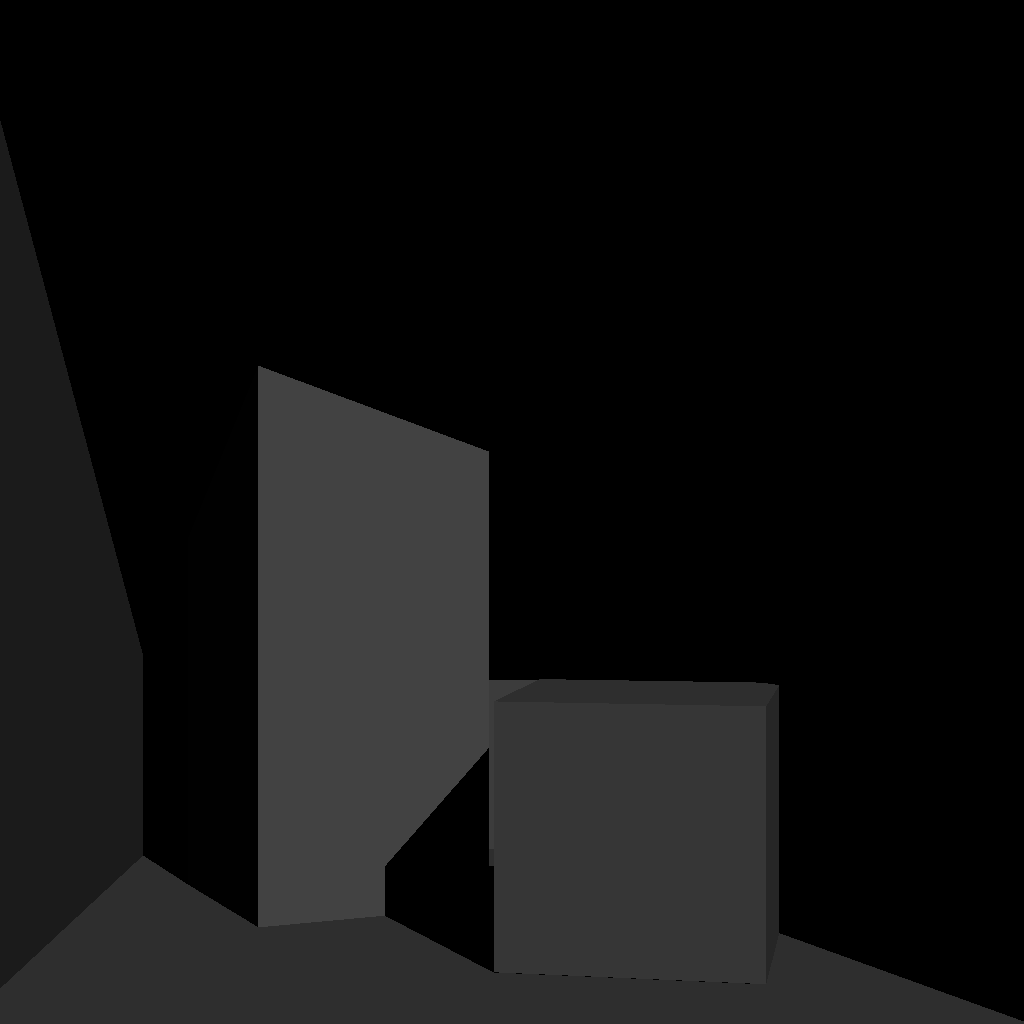
\includegraphics[width=\textwidth]{q1/CornellBox/directional_light.png}
        \caption{Rendering of CornellBox: Directional Light}
    \end{minipage}
    \hfill
    \begin{minipage}[t]{.4\textwidth}
        \centering
        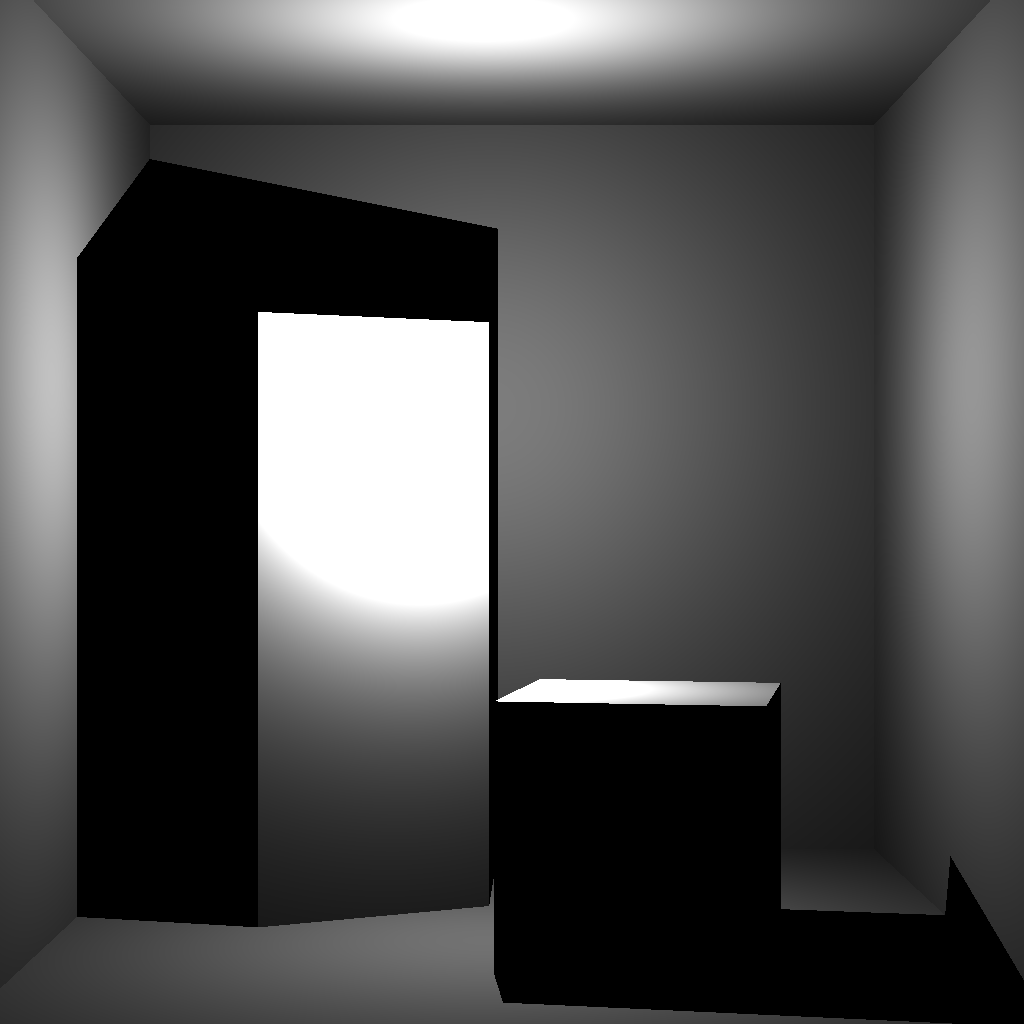
\includegraphics[width=\textwidth]{q1/CornellBox/point_light.png}
        \caption{Rendering of CornellBox: Point Light}
    \end{minipage}
\end{figure}

\begin{figure}[H]
    \begin{minipage}[t]{.4\textwidth}
        \centering
        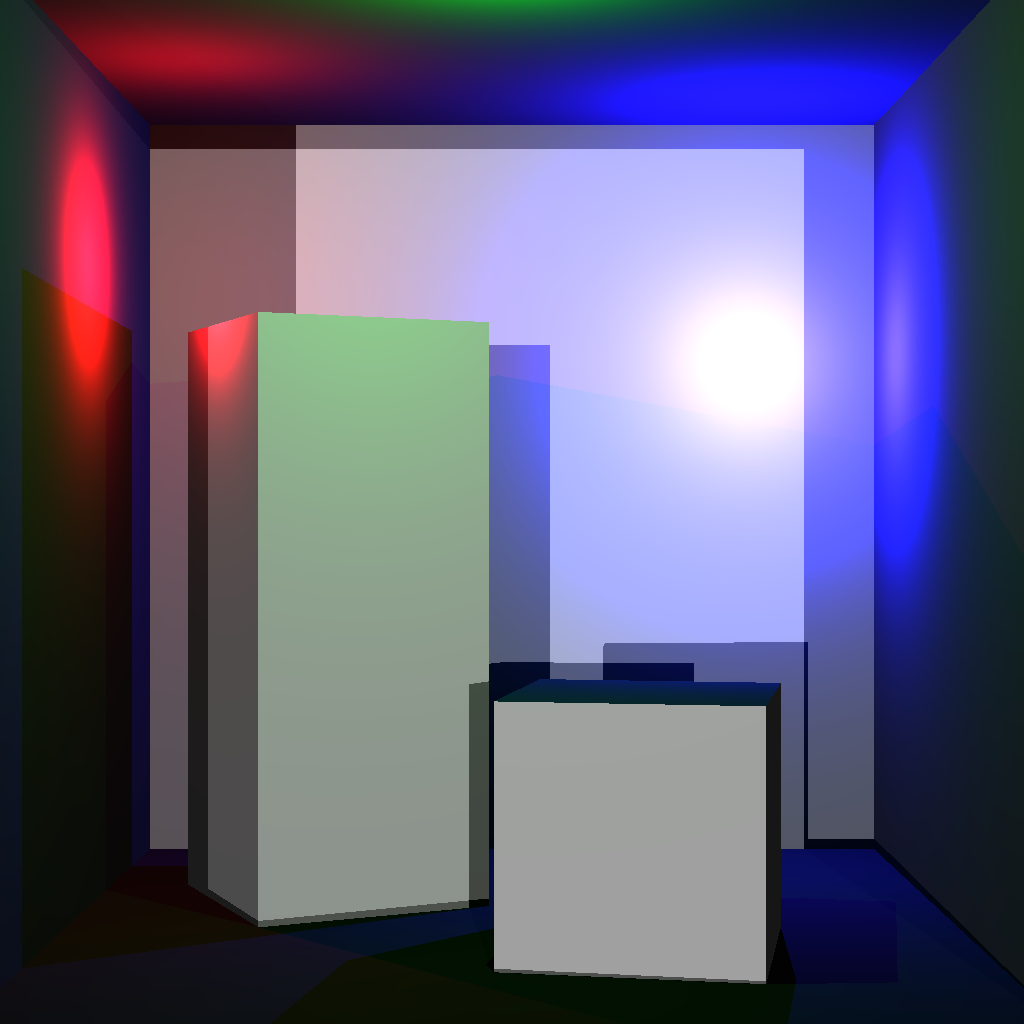
\includegraphics[width=\textwidth]{q1/CornellBox/many_lights.png}
        \caption{Rendering of CornellBox: Many Lights}
    \end{minipage}
    \hfill
    \begin{minipage}[t]{.4\textwidth}
        \centering
        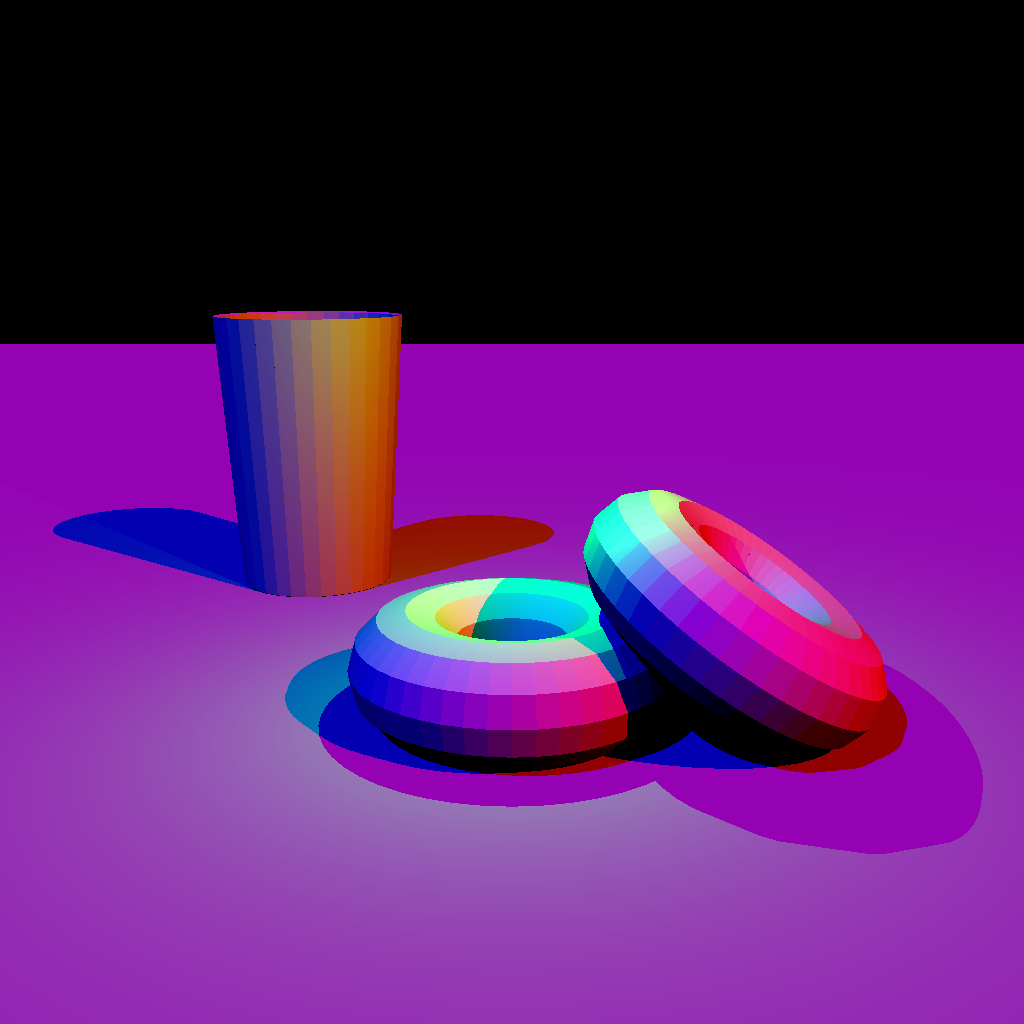
\includegraphics[width=\textwidth]{q1/Donuts/scene.png}
        \caption{Rendering of Donuts (Many Lights)}
    \end{minipage}
\end{figure}

\section{Texture Mapping}

\subsection{Timings}

\begin{table}[H]
\centering
\renewcommand{\arraystretch}{1.5}
\begin{tabularx}{\linewidth}{LL}
\hline
Scene & Render Time (ms) \\
\hline
CornellBox: Directional Light & 1264.921997 \\
CornellBox: Point Light & 1407.619019 \\
CornellBox: Many Lights & 2411.620117 \\
Donuts (Many Lights) & 2753.679932 \\
Monkey in the Woods (Many Lights) & 2112.415039 \\
\hline
\end{tabularx}
\caption{Time taken (in ms) for rendering models, with nearest neighbour texture map}
\end{table}

\subsection{Rendered Images}

\begin{figure}[H]
    \begin{minipage}[t]{.4\textwidth}
        \centering
        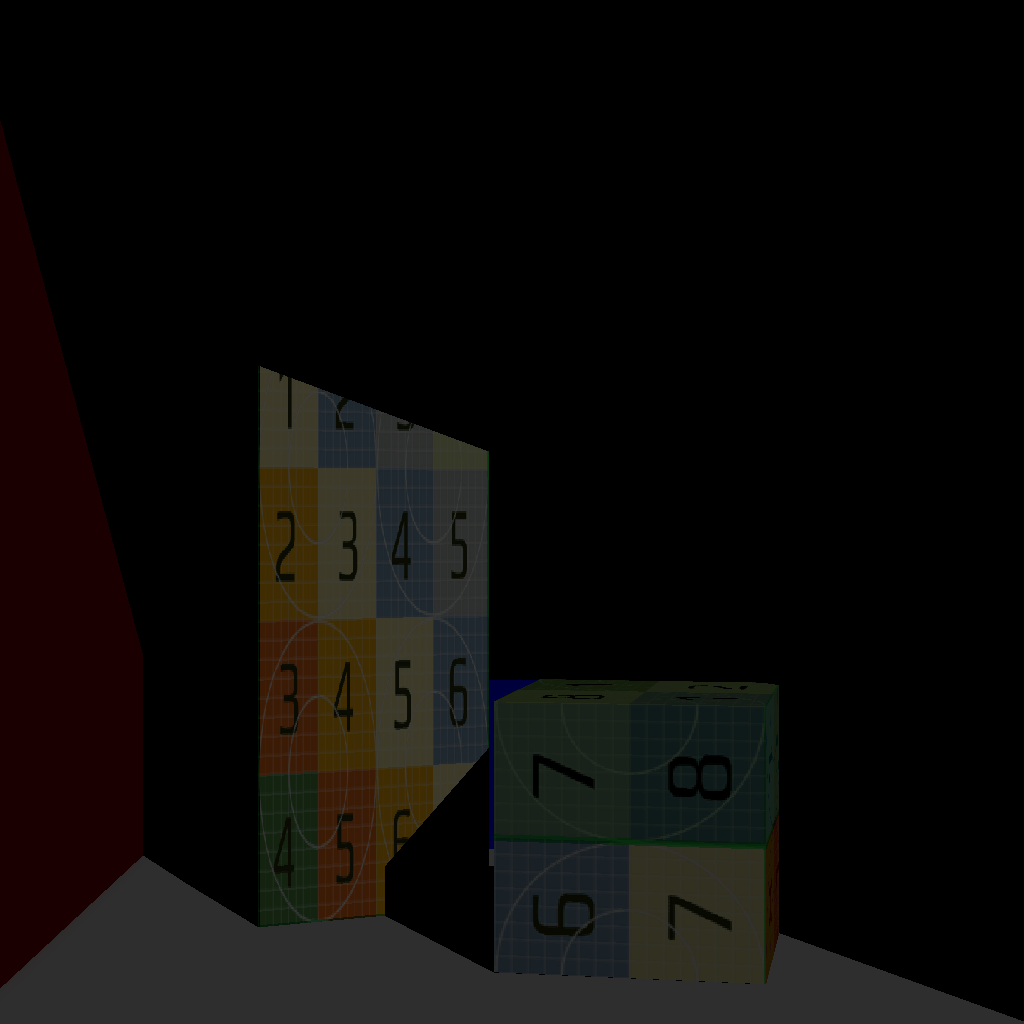
\includegraphics[width=\textwidth]{q2/CornellBox/directional_light.png}
        \caption{Rendering of CornellBox: Directional Light, with nearest neighbour texture map}
    \end{minipage}
    \hfill
    \begin{minipage}[t]{.4\textwidth}
        \centering
        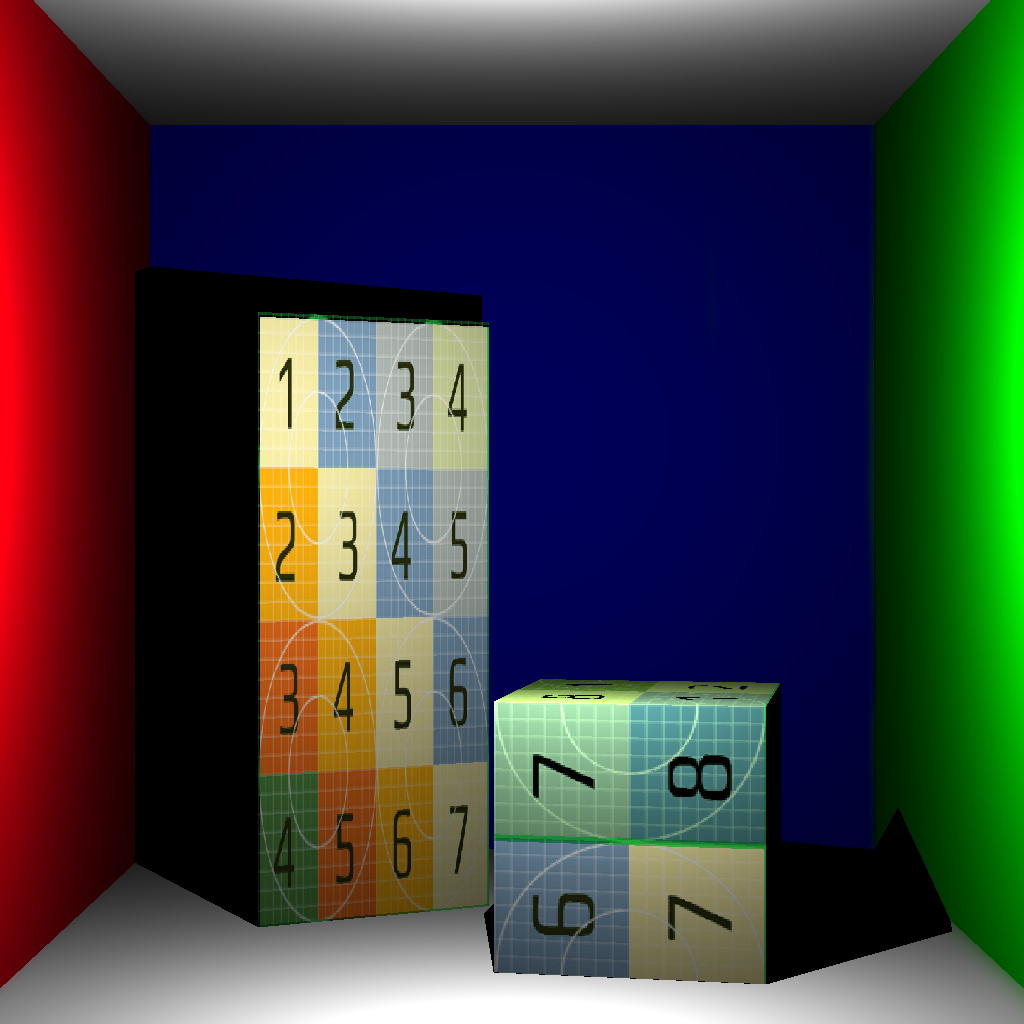
\includegraphics[width=\textwidth]{q2/CornellBox/point_light.png}
        \caption{Rendering of CornellBox: Point Light, with nearest neighbour texture map}
    \end{minipage}
\end{figure}

\begin{figure}[H]
    \begin{minipage}[t]{.4\textwidth}
        \centering
        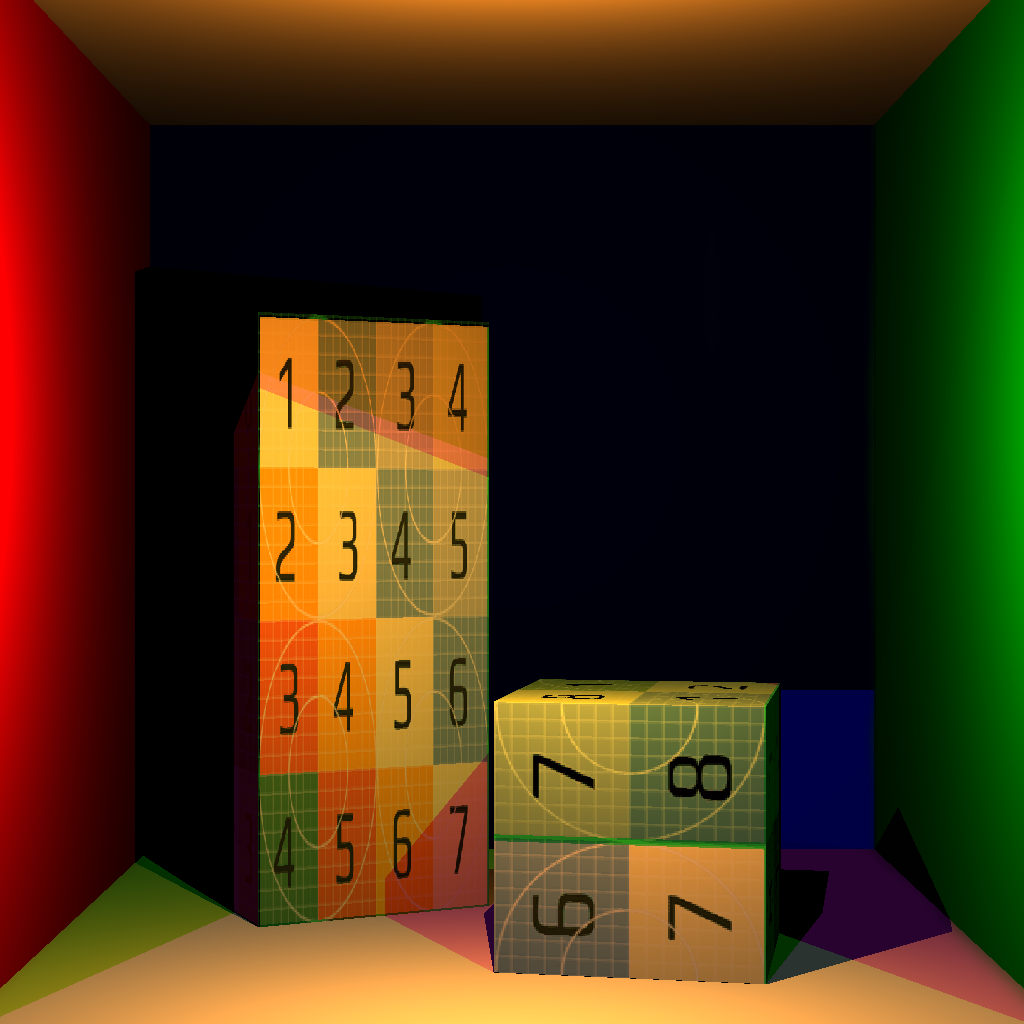
\includegraphics[width=\textwidth]{q2/CornellBox/many_lights.png}
        \caption{Rendering of CornellBox: Many Lights, with nearest neighbour texture map}
    \end{minipage}
    \hfill
    \begin{minipage}[t]{.4\textwidth}
        \centering
        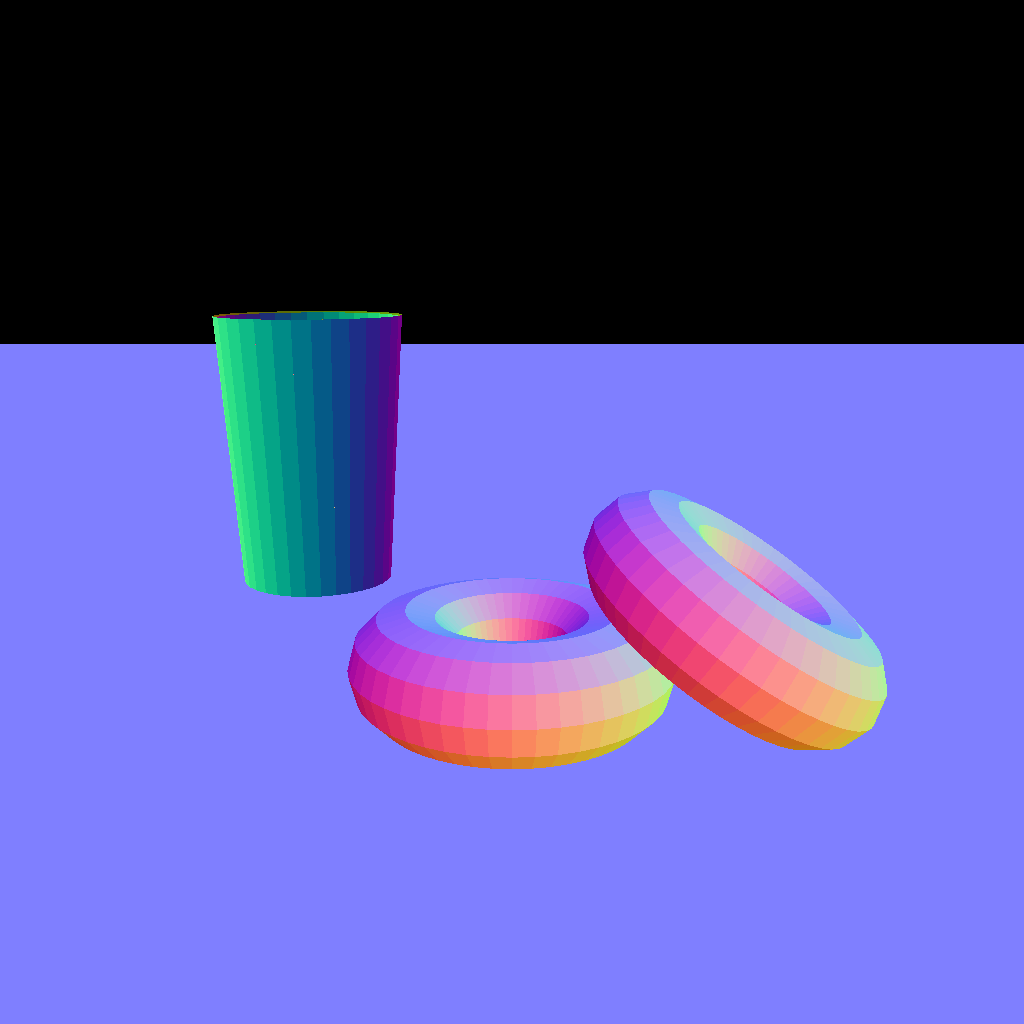
\includegraphics[width=\textwidth]{q2/Donuts/scene.png}
        \caption{Rendering of Donuts, with nearest neighbour texture map}
    \end{minipage}
\end{figure}

\begin{figure}[H]
    \centering
    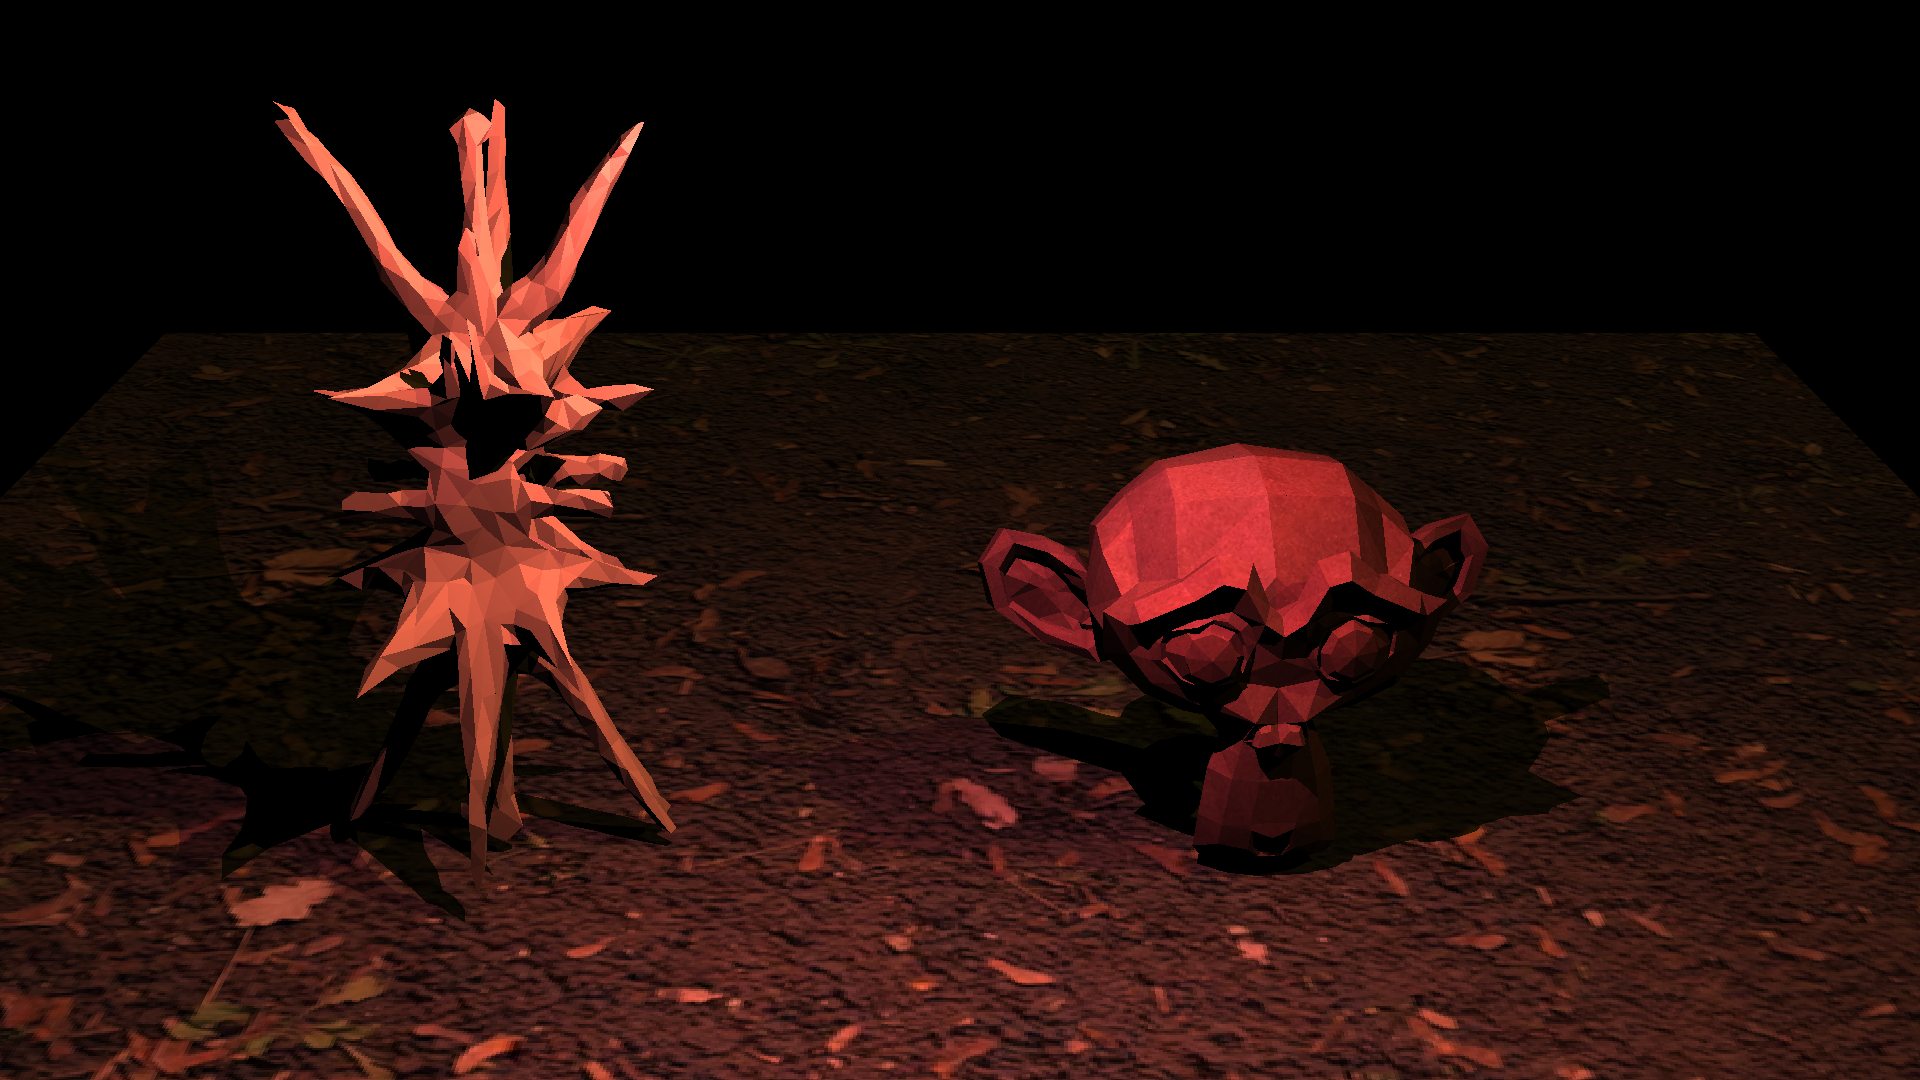
\includegraphics[width=.85\textwidth]{q3/scene.png}
    \caption{Rendering of Monkey in the Woods, with nearest neighbour texture map}
\end{figure}

\end{document}
